\documentclass{article}
\usepackage[utf8]{inputenc}
\usepackage[english]{babel}
\usepackage{hyperref}
\makeindex

\title{Foundations of Artificial Intelligence}
\author{Riccardo Salvalaggio}
\date{19th of April, 2021}

\usepackage{amssymb}
\usepackage{amsmath}
\usepackage{txfonts}
\usepackage{mathdots}
\usepackage[classicReIm]{kpfonts}
\usepackage{graphicx}

\begin{document}

\maketitle
\newpage
\tableofcontents
\newpage

\section{Introduction}
Artificial Intelligence is the attempt to make computers more "intelligent" to better understand human intelligence.
\section{Rational Agents}
It is a model that perceive the environment through sensors and act through actuators. In order to evaluate their performance use performance measure (e.g. vacuum -> level of cleanliness etc.) even if optimal behaviour is often unattainable because it is quite impossible to reach the goal in every aspect.\\ \textbf{Omniscent }if it knows the effects of its actions.\\ \textbf{Rational} agent behaves according to its percepts and knowledge and attempts to maximize the expected performance.\\ \textbf{Ideal: }for each possible percept sequence, selects an action that is expected to maximize its performance measure.
\subsection{Structure of Rational Agents}
The mapping is realised through an agent program executed on an Architecture which also provides an interface to the environment(percepts, actions)
\textbf{Agent = Architecture + Program}
\subsection{Classes of agents}
\subsubsection{Table-Driven (the simplest)}
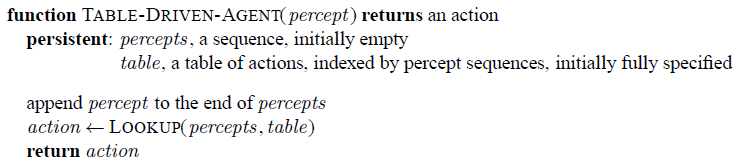
\includegraphics[scale=0.8]{1.png}
Problem: need a huge table to fulfill all the possible perceptions.\\
\newpage
\subsubsection{Interpretative Reflex}
\begin{figure}[h!]
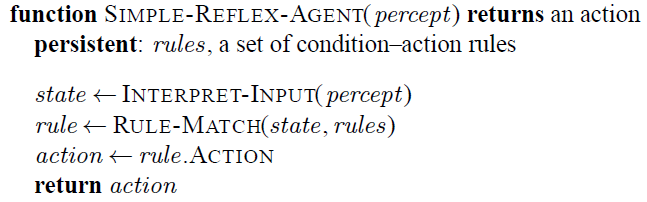
\includegraphics[scale=0.5]{2.png}
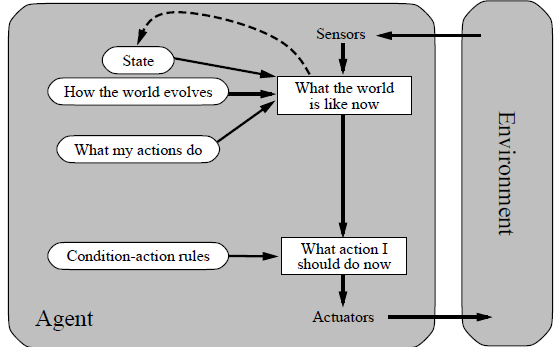
\includegraphics[scale=0.5]{3.png}
Interpretation of the input, matching to a rule to extract an action.
\end{figure}
\subsubsection{Model-Based Reflex}
\begin{figure}[h!]
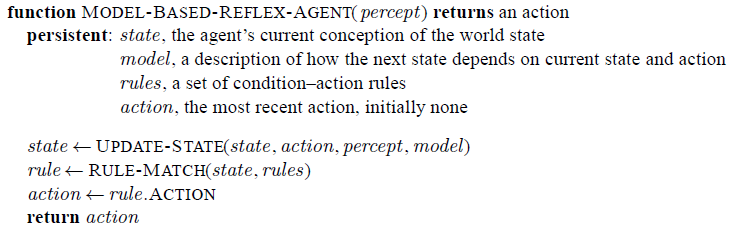
\includegraphics[scale=0.5]{4.png}
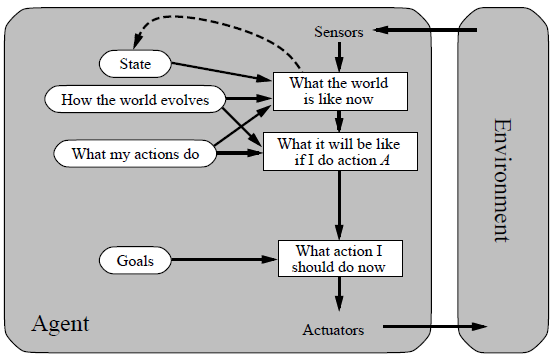
\includegraphics[scale=0.36]{5.png}
\caption{Goal-based}
\end{figure}
Introduction of a utlity function that maps a state onto a real number in order to compute the best action to do and to weigh the importance of competing goals.
\begin{figure}[h!]
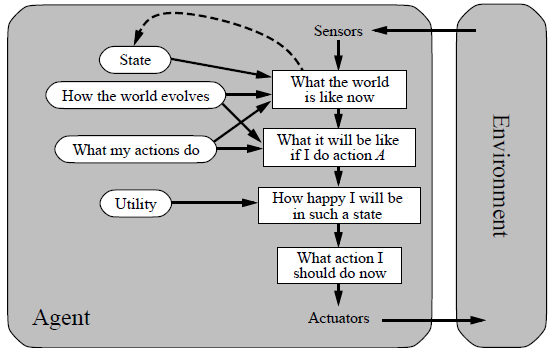
\includegraphics[scale=0.5]{6.png}
\caption{Utility-based}
\end{figure}
\subsubsection{Learning agents}
Agents that improve over time starting from an empty knowledge and unknown environments.\\
\textbf{Components: }\\
\textit{Learning element:} responsible for making improvements.\\
\textit{Performance element:} select external actions.\\
\textit{Critic: }determines performance of the agent.\\
\textit{Problem generator: }suggests actions that lead to informative experiences.\\
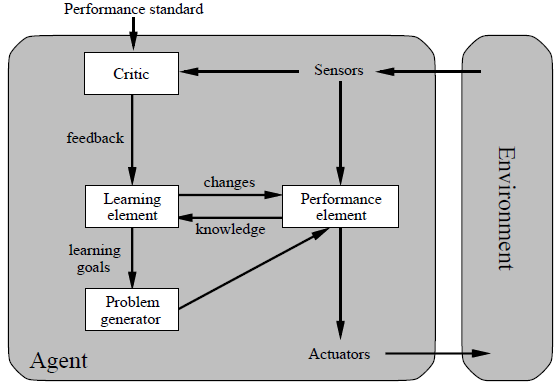
\includegraphics[scale=0.5]{7.png}
\subsection{Types of environments}
Accessible vs. inaccessible, Deterministic vs. stochastic, Episodic vs. sequential, static vs. dynamic, discrete vs. continuous, single vs. multi agent.

\section{Solving Poblems by Searching}
\subsection{Problem-solving agents}
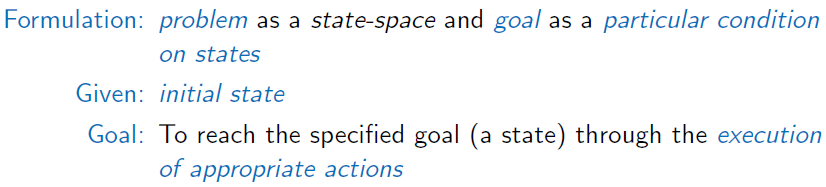
\includegraphics[scale=0.6]{8.png}\\
\begin{figure}
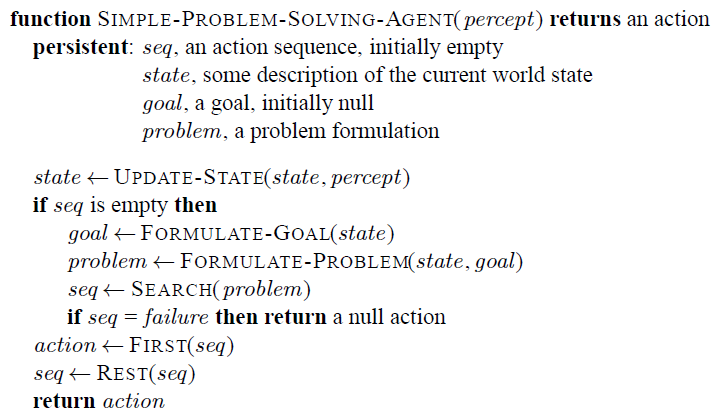
\includegraphics[scale=0.6]{9.png}\\
\caption{Simple Problem-solving Agent}
\end{figure}\\\\
- Properties: Fully-observable, Deterministic/static env., discrete states, single-agent.\\

\subsection{Problem Formulation}
Goal formulation, definition of: State space, actions, problem type, search and execution costs.\\
\subsection{Problem Types}
Based on knowledge of States and Actions: Observability, completeness of knowledge about world state and actions. (e.g. If the environment is completely observable, the vacuum cleaner always knows where it is and where the dirt is.)\\
Transition Model: Description of the outcome of an action.\\
Solution: Path from the initial to a goal state.\\
Search Costs: Time and storage requirements to and a solution.\\
Total Costs: Search costs + path costs.\\
Alternative formulations can influence a lot number of states, e.g. 8 queens problem: Naive - billions of state, Better - 2057 states.\\
Examples of Real-World Problems: Route planning, shortest path problem, TSP, VLSI Layout, Robot nav., Assembly sequencing.\\
\subsection{Search strategies}
E.g.: node expansion, frontier, search strategy, tree-based search, graph-based search.\\
- Search Tree Data structure:\\
state, parent, action, path-cost.\\

\begin{figure}[h!]
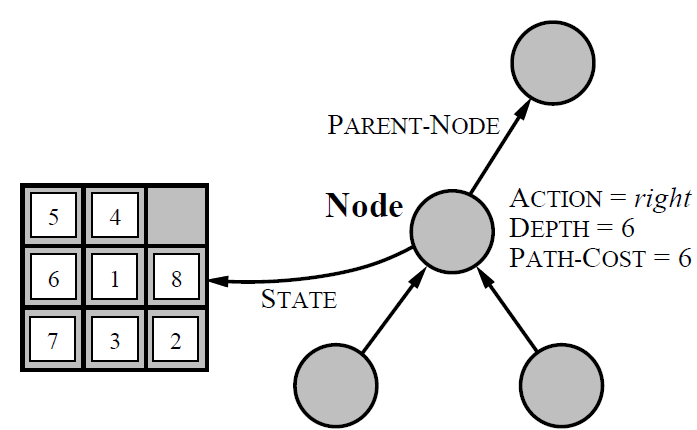
\includegraphics[scale=0.6]{10.png}
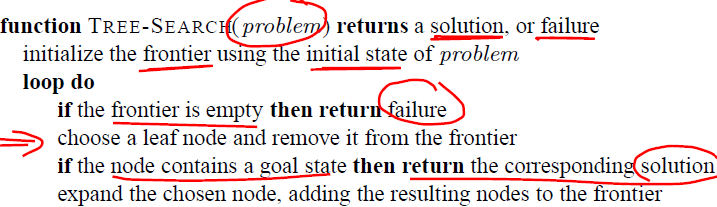
\includegraphics[scale=0.6]{11.png}
\end{figure}

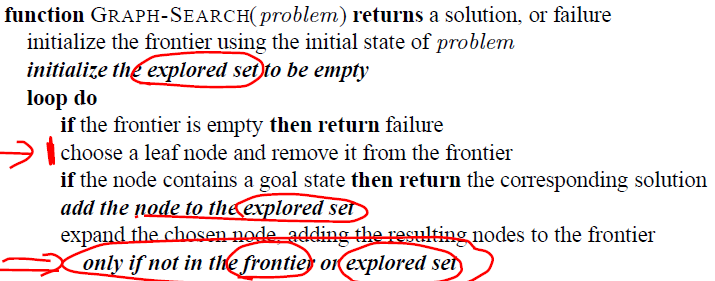
\includegraphics[scale=0.6]{12.png}\\\\
- Criteria for Search Strategies: \textbf{\textit{Completeness, Time complexity, Space Complexity, Optimality}}.\\

\subsubsection{Uninformed or blind searches}
- Breadth-First Search:\\
Nodes are expanded in the order they were produced (first siblings, then children) (frontier = FIFO queue). Completeness is obvious, the solution is optimal. \textbf{Time complexity: }Let b be the maximal branching factor and d the depth of a solution path. Then the maximal number of nodes expanded is = O(b at d).\textbf{ Space Complexity: O(b at d)}\\\\
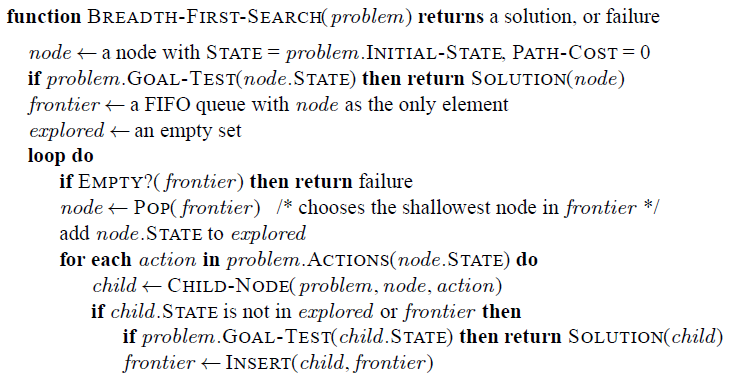
\includegraphics[scale=0.6]{13.png}\\\\
- Uniform-Cost Search:\\
If step costs are different, uniform cost is better. It expands node with lowest path costs \textit{g(n)}. It uses a Priority queue. Always finds the cheapest solution, given that g(successor(n)) $>=$ g(n) for all n.\\
- Depth-First Search:\\
Always expands an unexpanded node at the greatest depth (frontier $<-$ a LIFO queue, first children, then siblings). Usually implemented recursively.\\
Generally, optimal is not guaranteed. Completeness only for graph-based search. \textbf{Time complexity: }in graph-based is bounded by the space, so it can be infinite, in tree-based: O(b at m) (m max length of a path). \textbf{Space Complexity: }tree-based: O(b*m), graph-based: worst-case, all states need to be stored. (no better than breadth-first).\\\\
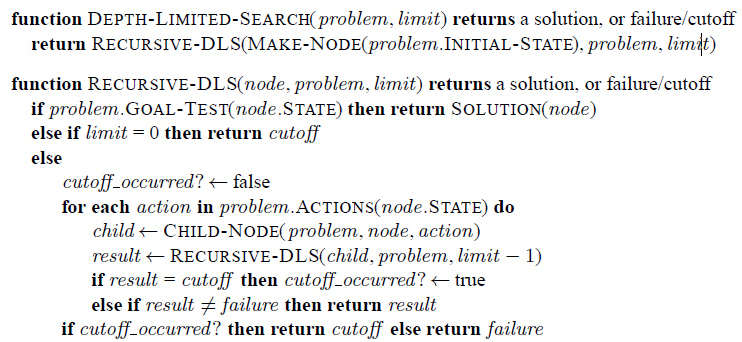
\includegraphics[scale=0.6]{14.png}\\\\
- Iterative Deepening Search:\\
Like depth-limited search and in every iteration increase search depth by one. Combines depth and breadth-first. Optimal and complete like breadth-first, but requires much less memory: O(b*d).\\\\
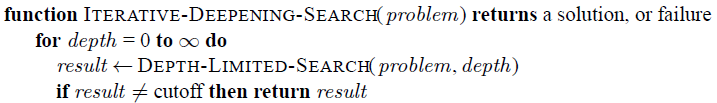
\includegraphics[scale=0.6]{15.png}\\\\
Iterative deepening in general is the preferred uninformed search method when there is a large search space and the depth of the solution is not known.\\
For small space it is worse than breadth-fist.\\
- Bidirectional searches:\\
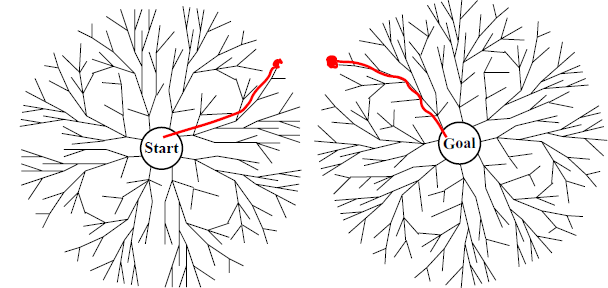
\includegraphics[scale=0.6]{16.png}\\\\
As long as forward and backward searches are symmetric, search times of O(2*b at d/2) = O(b at d/2) can be obtained. The operators are not always reversible, there must be an efficient way to check if a new node already appears in the search tree of the other half of the search.\\
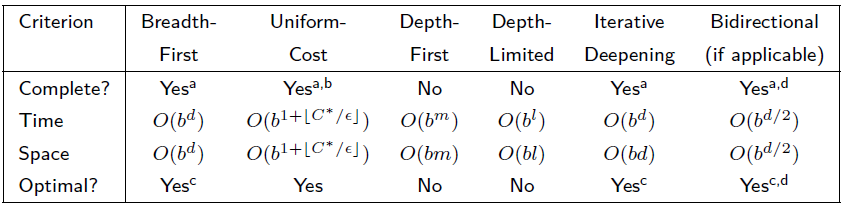
\includegraphics[scale=0.6]{17.png}

\section{Informed Search Methods}
- Uninformed: rigid procedure with no knowledge of the cost of a given node to the goal.\\
- Informed: knowledge of the worth of expanding a node n is given in the form of an evaluation function f(n) which assigns a real number to each node. Mostly,
f(n) includes as a component a heuristic function h(n), which estimates the costs of the cheapest path from n to the goal.\\
- Best-first: informed that expands with the best f-value.\\\\
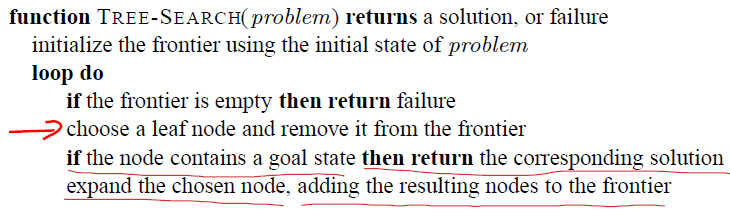
\includegraphics[scale=0.6]{18.png}
Instance of tree-search algorithm in which frontier is a priority queue. When f is always correct, we don't need to search.\\
\subsection{Greedy Search}
h(n) = estimated path-costs from n to the goal. A best-first search using h(n) (heuristic function) as evaluation function is called greedy search.
\subsection{Heuristics}
Heuristics are fast but in certain situations incomplete methods for problem-solving, they improve the search in the average-case and the time complexity. In general, not optimal and incomplete; graph-search version is complete only in finite spaces.
\subsection{A* and IDA*}
A* combines greedy search with the uniform-cost search: always expand node with lowest f(n) = g(n) (actual cost from start to n) + h(n) (estimated cost to goal/optimistic estimate of the costs). A new h is \textit{admissible} iff: h(n) $<=$ h*(n).
\subsubsection{Optimality of A*}
\textbf{Claim: }The first solution found has the minimum path cost.\\
\textbf{Proof: }Suppose there exists a goal node G with optimal path cost f*, but
A* has first found another node G2 with g(G2) > f*. Let n be a node on the path from the start to G that has not yet been expanded. Since h is admissible, we have: f(n)$<=$f* $-->$ f(G2)$<=$f(n) $-->$ f(G2)$<=$f* $==>$ g(G2)$<=$f* Contraddiciton.\\
- Completeness: If a solution exists, A* will find it provided that (1) every node has a finite number of successor nodes, and (2) there exists a positive constant $\delta$ > 0 such that every step has at least cost $\delta$.\\
- Complexity: In general, still exponential in the path length of the solution (space, time), it depends on the choice of Heuristic used.
\subsubsection{Graph- vs. Tree-search}
For the graph-based variant, either needs to consider re-opening nodes from the explored set, when a better estimate becomes known, or needs to require stronger restrictions on the heuristic estimate: it needs to be consistent (iff for all actions a leading from s to s': h(s) - h(s') $<=$ c(a), where c(a) denotes the cost of action a). Consistency implies admissibility, A* can still be applied if heuristic is not consistent but optimality is lost.
\subsubsection{Variants of A*}
In general suffers from exponential memory growth.
- Iterative-deepening A*: f-costs are used to define the cut-off (IDA*).\\
- Recursive Best First Search (RBFS): introduces a variable \textit{f-limit} to
keep track of the best alternative path, if the limit is exceeded opt for the alternative path.\\
- MA* and SMA*.

\subsection{Local Search Methods}








\end{document}
